% ****** Start of file apssamp.tex ******
%
%   This file is part of the APS files in the REVTeX 4.2 distribution.
%   Version 4.2a of REVTeX, December 2014
%
%   Copyright (c) 2014 The American Physical Society.
%
%   See the REVTeX 4 README file for restrictions and more information.
%
% TeX'ing this file requires that you have AMS-LaTeX 2.0 installed
% as well as the rest of the prerequisites for REVTeX 4.2
%
% See the REVTeX 4 README file
% It also requires running BibTeX. The commands are as follows:
%
%  1)  latex apssamp.tex
%  2)  bibtex apssamp
%  3)  latex apssamp.tex
%  4)  latex apssamp.tex
%
\documentclass[%
 reprint,
%superscriptaddress,
%groupedaddress,
%unsortedaddress,
%runinaddress,
%frontmatterverbose, 
%preprint,
%preprintnumbers,
%nofootinbib,
%nobibnotes,
%bibnotes,amsmath, amssymb, aps,
%pra,
%prb,
%rmp,
%prstab,
%prstper,
%floatfix,
]{revtex4-2}

	


\usepackage{graphicx}% Include figure files
\usepackage{dcolumn}% Align table columns on decimal point
\usepackage{bm}% bold math
\usepackage{setspace}
\usepackage{amsmath, xparse}
%\usepackage{hyperref}% add hypertext capabilities
%\usepackage[mathlines]{lineno}% Enable numbering of text and display math
%\linenumbers\relax % Commence numbering lines

%\usepackage[showframe,%Uncomment any one of the following lines to test 
%%scale=0.7, marginratio={1:1, 2:3}, ignoreall,% default settings
%%text={7in,10in},centering,
%%margin=1.5in,
%%total={6.5in,8.75in}, top=1.2in, left=0.9in, includefoot,
%%height=10in,a5paper,hmargin={3cm,0.8in},
%]{geometry}

\onehalfspacing

\begin{document}

\preprint{APS/123-QED}

\title{Modelling Covid-19 Immunity Dynamics in Chapel Hill, NC \\ using an Adjusted SIR Model}% Force line breaks with \\


\author{Ariba Huda}
\affiliation{
 University of North Carolina at Chapel Hill, Department of Mathematics \\
 MATH 528: Mathematical Methods in Physical Sciences% with \\
}%


\date{\today}% It is always \today, today,
             %  but any date may be explicitly specified

\begin{abstract}

Mathematical modeling and ordinary differential equations (ODEs) are a key tool used in epidemiology to model infectious disease spread in populations. There are many existing ODEs that aim to model rate of infection in a population under limiting assumptions. These models typically measure the number of susceptible, infected, and recovered individuals under the assumption that a population remains fixed and immunity is permanent. More recent adaptations of these models factor in birth, death, and exposure latency rate. However, as seen through the recent spread of COVID-19 variants, there is a necessity to consider that those who have recovered from COVID-19 can be susceptible for reinfection. This project proposes a model that incorporates an immunity loss rate variable in a typical disease spread ODE to better model and predict endemic equilibrium.

\begin{description}
\item[Code]
Code for simulations can be found at https://github.com/ar1ba/CovidModel-Math528.
 
\end{description}
\end{abstract}

%\keywords{Suggested keywords}%Use showkeys class option if keyword
                              %display desired
\maketitle

%\tableofcontents

\section{\label{sec:level1}Introduction\protect\\}

As a Biostatistics major taking this mathematical modeling course as a degree requirement, I have been interested in combining concepts we have used to model phenomena in the physical sciences to my background in public health—specifically within disease modeling. One branch of public health that utilizes differential equations heavily is epidemiology and there are various models already created to model disease spread across populations. The SIR model, specifically, is a commonly used compartmental model in epidemiology which categorizes population classes into the susceptible, infective, and recovered. A more recent application of the SIR model is used to understand COVID-19 disease dynamics. However, the SIR model has the limitation of assuming recovered individuals of COVID-19 have permanent immunity to the disease. Due to the rapid manifestation of COVID-19 variants and uncertainty of immunity within many recovered individuals, there could be great use in adapting the SIR model to consider the possibility of immunity loss post-recovery. I am interested in independently creating an adapted-SIR model so that, for simplicity, researchers can still predict disease dynamics even if they do not have available current data on exposed populations, latency periods, and birth and death rates.

\section{\label{sec:level1}The SIR Model for Disease Spread\protect\\}

From the classic work on the theory of epidemics done by Kermack and McKendrick in 1927, we begin with a deterministic model that derives an approximate solution for the infection rate of susceptible populations, spread rate of infected populations, and removal rate of recovered populations. We have to make a couple of assumptions: the population is fixed, recovery results in immunity, the incubation period is close to negligible, and the various groups are uniformly mixed. These are given in a set of nonlinear ODEs that represent continuous changes over time with the initial conditions $S(0)=S_0>0, I(0)=I_0>0, R(0)=0$.

\begin{equation} \frac{dS}{dt} = \frac{-aSI}{N} \end{equation}
\begin{equation} \frac{dI}{dt} = \frac{aSI}{N} - bI \end{equation}
\begin{equation} \frac{dR}{dt} = bI \end{equation}

The units for a/N are $(time-per-individual)^-1$ and it measures the proportionality constant for the gain in infected individuals and the product of susceptible and infected classes, $a>0$. The units for b are $(time)^-1$ and measures the treatment rate of the infected class, $b>0$. 

Because we assume population is fixed, by our initial conditions, the total population can be written as $N_0=S_0+I_0$. The reproductive rate of infection is R(0)=0, so the model can be given in just S(t) and I(t). We rewrite I as a function of S using equations (1) and (2):

\begin{equation} \frac{dI}{dS} = \frac{-aSI-bI}{-aSI} = (-1-\frac{b}{aS}) = -1+\frac{\rho}{S} \end{equation} where $I \neq 0$ and $\rho=\frac{b}{a}$

\section{\label{sec:level1}Adjusting the SIR Model to incorporate immunity loss variable ($\omega$)\protect\\}

Using the SIR Model as a framework, I propose an adjusted model that considers the possibility of immunity loss in COVID-19. With initial conditions $S(0)\geq0, I(0)\geq0, R(0)\geq0$, and total population $N=S+I+R$:

\begin{equation} \frac{dS}{dt} = \frac{-aSI}{N} + \omega(N-(S+I)) \end{equation}
\begin{equation} \frac{dI}{dt} = \frac{aSI}{N} - bI \end{equation}
\begin{equation} \frac{dR}{dt} = bI - \omega(N-(S+I)) \end{equation}

This adjusted model similarly uses $\frac{-aSI}{N}$ to measure the number of infections caused per infected individuals per time and $b$ measures the treatment and recovery rate of the population over time. We now include $\omega$, our rate of immunity loss over time, which is multiplied by the number of recovered individuals in terms of N, S and I, and is re-added back to our model for the susceptible population (5), and subtracted from our current recovered population (7). This is because individuals who have lost their immunity are no longer classified as recovered but now back to being susceptible for reinfection of COVID-19. 

Similarly to the SIR model, it is sufficient to only consider equations (5) and (6) as R(t) can be directly obtained from S(t) and I(t). 

Lastly, we can apply forward Euler’s Formula in order to separate the first step size and obtain the following solutions:

\begin{equation} S_t_+_1 = S_t + \delta(\frac{-aS_tI_t}{N} + \omega(N-(S_t + I_t))) \end{equation}
\begin{equation} I_t_+_1 = I_t + \delta(\frac{-aS_tI_t}{N} - bI) \end{equation}

\section{\label{sec:level1}Determining Existence of Equilibrium Points in New System\protect\\}

To determine the equilibrium solutions of our model, we must find all pairs (S,I) that result in S’=I’=0. 

To do this I set (5) equal to 0 and get $S'=0=-aSI + N^2\omega - NS\omega - NI\omega$.
When solving for the roots of $S'$, I get that when $S=S, I=\frac{N(N-S)\omega}{Sa+N\omega}$ and when $I=I, S=\frac{N(N-I)\omega}{Ia+N\omega}$.

Next, I set (6) equal to 0 and get $I'=0=asI-NbI$. When solving for roots, I get that when $S=S, I=0$ and when $I=I, S=\frac{Nb}{a}$.

Thus, we get the following critical points:
\begin{equation} S=\frac{N(N-1)\omega}{Ia+N\omega}, I=0 \rightarrow (\frac{N^2\omega}{N\omega},0) = (N,0)  \end{equation}

\begin{equation} \label{eqn:CP2} S_e=\frac{Nb}{a}, I_e=\frac{N(N-S)\omega}{Sa+N\omega} \rightarrow (\frac{Nb}{a},\frac{N(a-b)\omega}{a(b+\omega)}) \end{equation}

From context, we know that critical point (10) represents a disease free equilibrium state where the total population is susceptible but none are infected yet. Thus, critical point (11) represents the equilibrium state during endemic conditions.

Let us consider the model from a system consisting of (8) and (9) and compute the Jacobian Matrix. \\

\begin{equation}
J(S,I) = 
\begin{bmatrix}
1+\delta(\frac{-aI}{N}-\omega)  &   -\delta(\frac{aS}{N}+\omega)\\
\delta(\frac{aI}{N})    &   1+\delta(\frac{aS}{N}-b) 
\end{bmatrix}
\end{equation}

Inserting our endemic equilibrium point (11) into the Jacobian matrix, we find

\begin{equation}
J(\frac{Nb}{a},\frac{N(a-b)\omega}{a(b+\omega)}) = \\ \begin{bmatrix} 
1+\delta\omega(\frac{a+\omega}{b+\omega}) & -\delta(b+\omega) \\
\delta\omega(\frac{a-b}{b+\omega}) & 1 \end{bmatrix}
\end{equation}

Then, we evaluate the trace and determinant of the Jacobian matrix at endemic equilibrium (13): \\

$T=Trace[J(S_e,I_e)]=2-\delta\omega(\frac{a+\omega}{b+\omega})$ \\
$D=Det[J(S_e,I_e)]=1-\delta\omega(\frac{a+\omega}{b+\omega}) + \delta^2\omega(a-b)$\\

Lastly, we compute the characteristic polynomial of the matrix at endemic equilibrium: \\

$\begin{vmatrix} J(S_e,I_e)-\lambda I\end{vmatrix} = \lambda^2 - \lambda(2-\delta\omega(\frac{a+\omega}{b+\omega}))+1-\delta\omega(\frac{a+\omega}{b+\omega}) + \delta^2\omega(a-b)=0$ \\

Using this polynomial, we can solve for $\lambda_1_,_2$ and evaluate stability at the equilibrium point.


\section{\label{sec:level1}Classifying Stability at Endemic Equilibrium Point \protect\\}

We can rewrite our Jacobian Matrix at endemic equilibrium $(S_e_q,I_e_q)$ (13) as so: \\

\begin{equation}
J(S_e_q,I_e_q) = \begin{bmatrix} 
1+\delta a_1_1 & -\delta a_1_2 \\
\delta a_2_1 & 1 \end{bmatrix}
\end{equation} \\

Thus, $T=2+\delta a_1_1$ and $D=1+\delta_a_1_1 + \delta^2a_1_2 a_2_1$. Our characteristic equation then becomes $\lambda^2 - T\lambda + D = 0$ and our roots result to: \\

\begin{equation}
\lambda_1_,_2 = \frac{2+\delta a_1_1}{2} \pm \frac{\delta}{2}\sqrt{a_1_1^2 - 4a_1_2 a_2_1}
\end{equation} \\

Stability of this system can be classified in 3 different cases. 
Case 1: $D = 1 + \delta a_1_1 + \delta^2 a_1_2 a_2_1 < 0$ results in an unstable saddle point where $\lambda_1_,_2$ are real and have different signs. \\

Case 2: $D = 1 + \delta a_1_1 + \delta^2 a_1_2 a_2_1 > 0$ results in 4 sub-cases. When $T^2-4D>0$, $\lambda_1_,_2$ are real with the same sign, and either results in a stable node $(T<0)$ and unstable node $(T>0)$. When $T^2-4D<0$, $\lambda_1_,_2$ are complex conjugates and result in a stable spiral $(T<0)$ or unstable spiral $(T>0)$. When $T^2-4D=0$, $\lambda_1_,_2$ are repeated real values and result in a stable degenerate sink $(T<0)$ or unstable degenerate sink $(T>0)$. Lastly, when $T=0$, $\lambda_1_,_2$ are pure imaginary values and result in a neutrally stable center. \\

Case 3: $D=0$ results in a line of fixed points or "comb" where $\lambda_1_,_2 = 0,T$ and is stable if $T<0$ or unstable if $T>0$.\\

\section{\label{sec:level1}Simulating Model with Parameters Based on COVID-19 data in Chapel Hill, NC\protect\\}

Using the Centers for Disease Control and Prevention (CDC)'s COVID Data Tracker, I collected relevant data on infection and treatment rates in Orange County in 2021 and utilized an approximate COVID immunity loss rate value based on average antibody and vaccine efficacy from an article in Nature. Our total population number is derived from the U.S. Census Bureau database. Specific parameters are listed in each figure caption. 


\begin{figure}[h]
\caption{Modelling 2021 Orange County COVID Data}
\centering
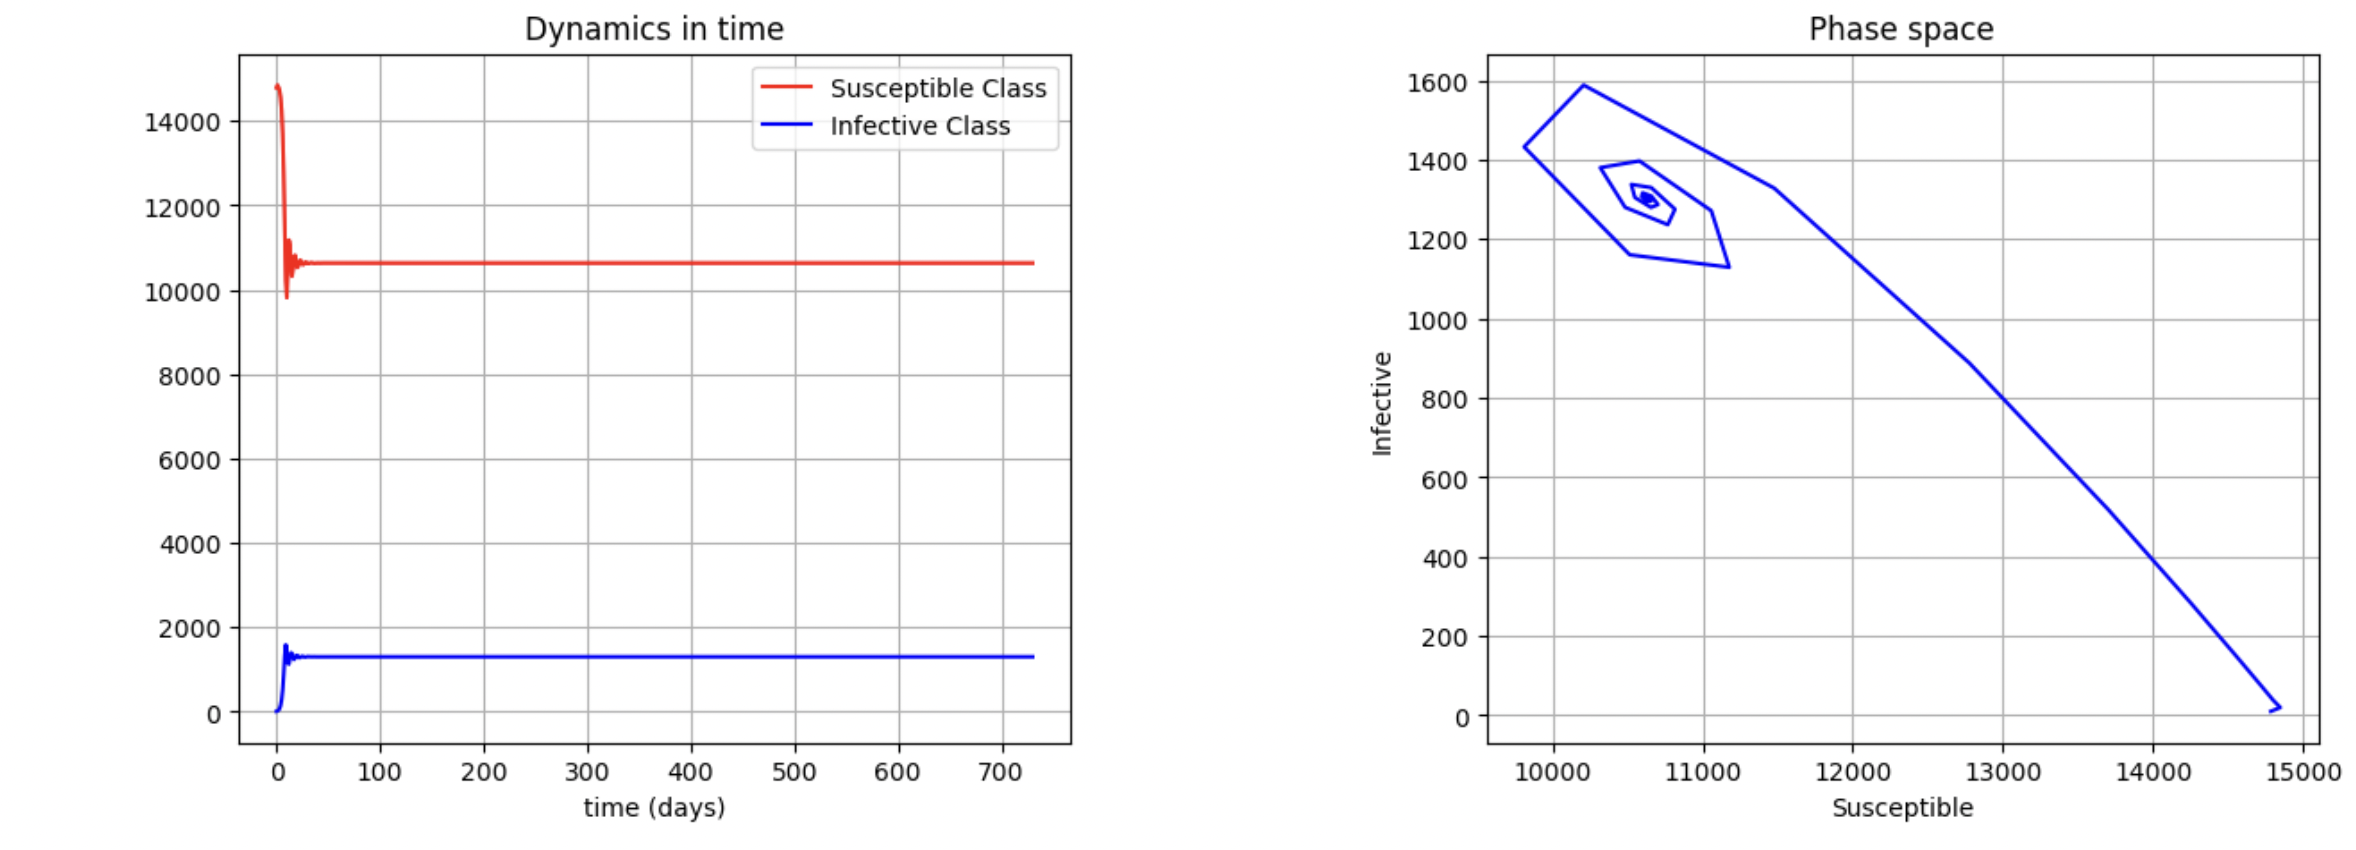
\includegraphics[width=80mm,scale=0.5]{2021-OrangeCountyData.png}
\end{figure}

Above, we model existing 2021 Covid-19 data in Orange County $(N=14,884, a=0.84,b=0.4, \omega = 0.265, \delta = 3.65)$. Our endemic equilibrium point $(S_e,I_e) = (3544, 6463)$ results in the following Jacobian Matrix: \\
\begin{equation}
J(S_e,I_e) = \begin{bmatrix} 
3.30 & -1.70 \\
1.33 & 1 \end{bmatrix}
\end{equation} \\
Here $T=-0.30$, $D=2.69$, and $T^2-4D=-10.67$ thus follows case 2, where $\lambda_1_,_2$ are complex conjugates. This model results in a stable spiral. \\

For the next couple of simulations, I take a random subset of the population data $(N=100)$ to better image immunity dynamics. The $a, b, \omega$ values remain constant to the 2021 Orange County data, however, now I explore the effects of altering the $\delta$ value.

\begin{figure}[h]
\caption{Modelling Subset Population COVID Data $(\delta = 2)$}
\centering
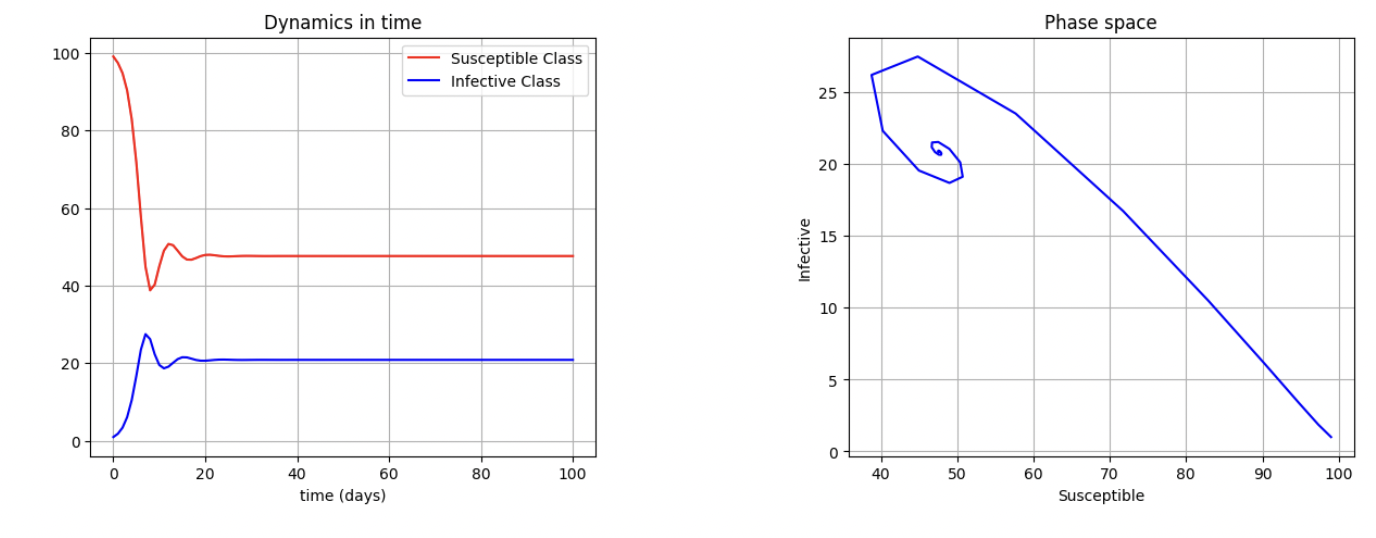
\includegraphics[width=80mm,scale=0.5]{n=100,a=.84,b=.4,d=2.png}
\end{figure}

Modelling subset $(N=100)$ data using $\delta = 2$, our endemic equilibrium point is $(S_e, I_e)= (47.6,20.9)$, and our following Jacobian Matrix is: 

\begin{equation}
J(S_e,I_e) = \begin{bmatrix} 
2.76 & -1.33 \\
0.35 & 1 \end{bmatrix}
\end{equation} \\

Here $T=3.76$, $D=3.23$, and $T^2-4D=1.24$ thus follows case 2 and our previous model, where $\lambda_1_,_2$ are real with the same sign. This model results in an unstable node. \\

\begin{figure}[h]
\caption{Modelling Subset Population COVID Data $(\delta = 3.6)$}
\centering
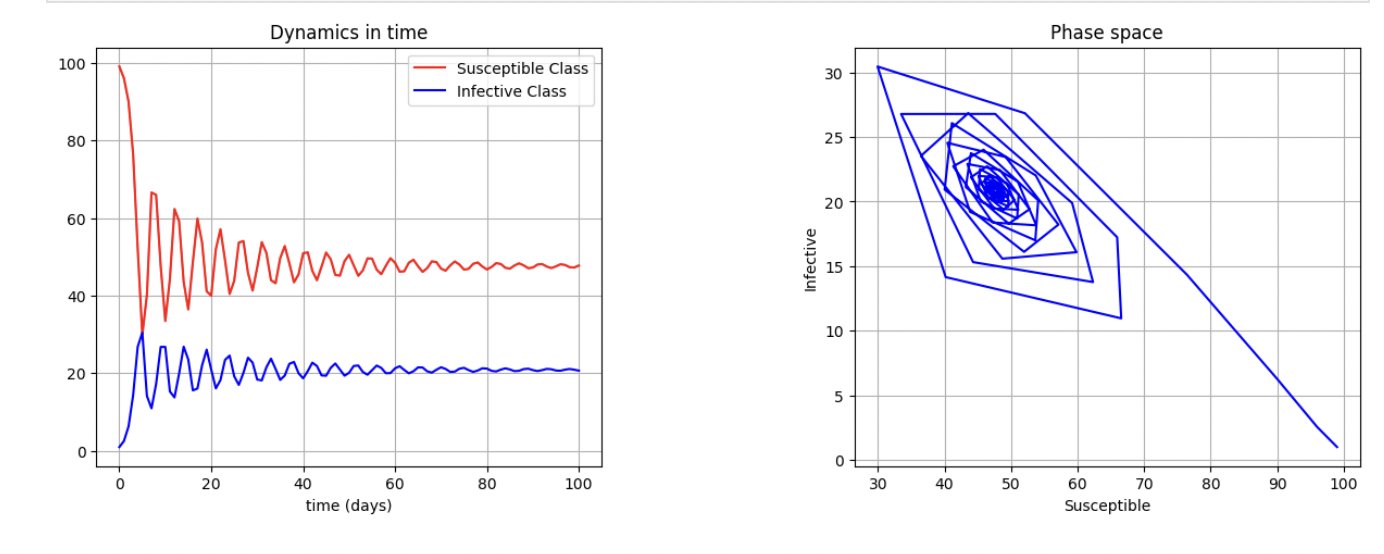
\includegraphics[width=80mm,scale=0.5]{n=100,a=.84,b=.4,d=3.6.png}
\end{figure}

Modelling subset $(N=100)$ data using $\delta = 3.6$, our endemic equilibrium point is $(S_e, I_e)= (47.6,20.9)$, and our following Jacobian Matrix is: 

\begin{equation}
J(S_e,I_e) = \begin{bmatrix} 
6.87 & -2.43 \\
0.64 & 1 \end{bmatrix}
\end{equation} \\

Here $T=7.87$, $D=8.42$, and $T^2-4D=28.2$ thus follows case 2 and our previous model, where $\lambda_1_,_2$ are real with the same sign. This model results in an unstable node. \\

\begin{figure}[h]
\caption{Modelling Subset Population COVID Data $(\delta = 4.5)$}
\centering
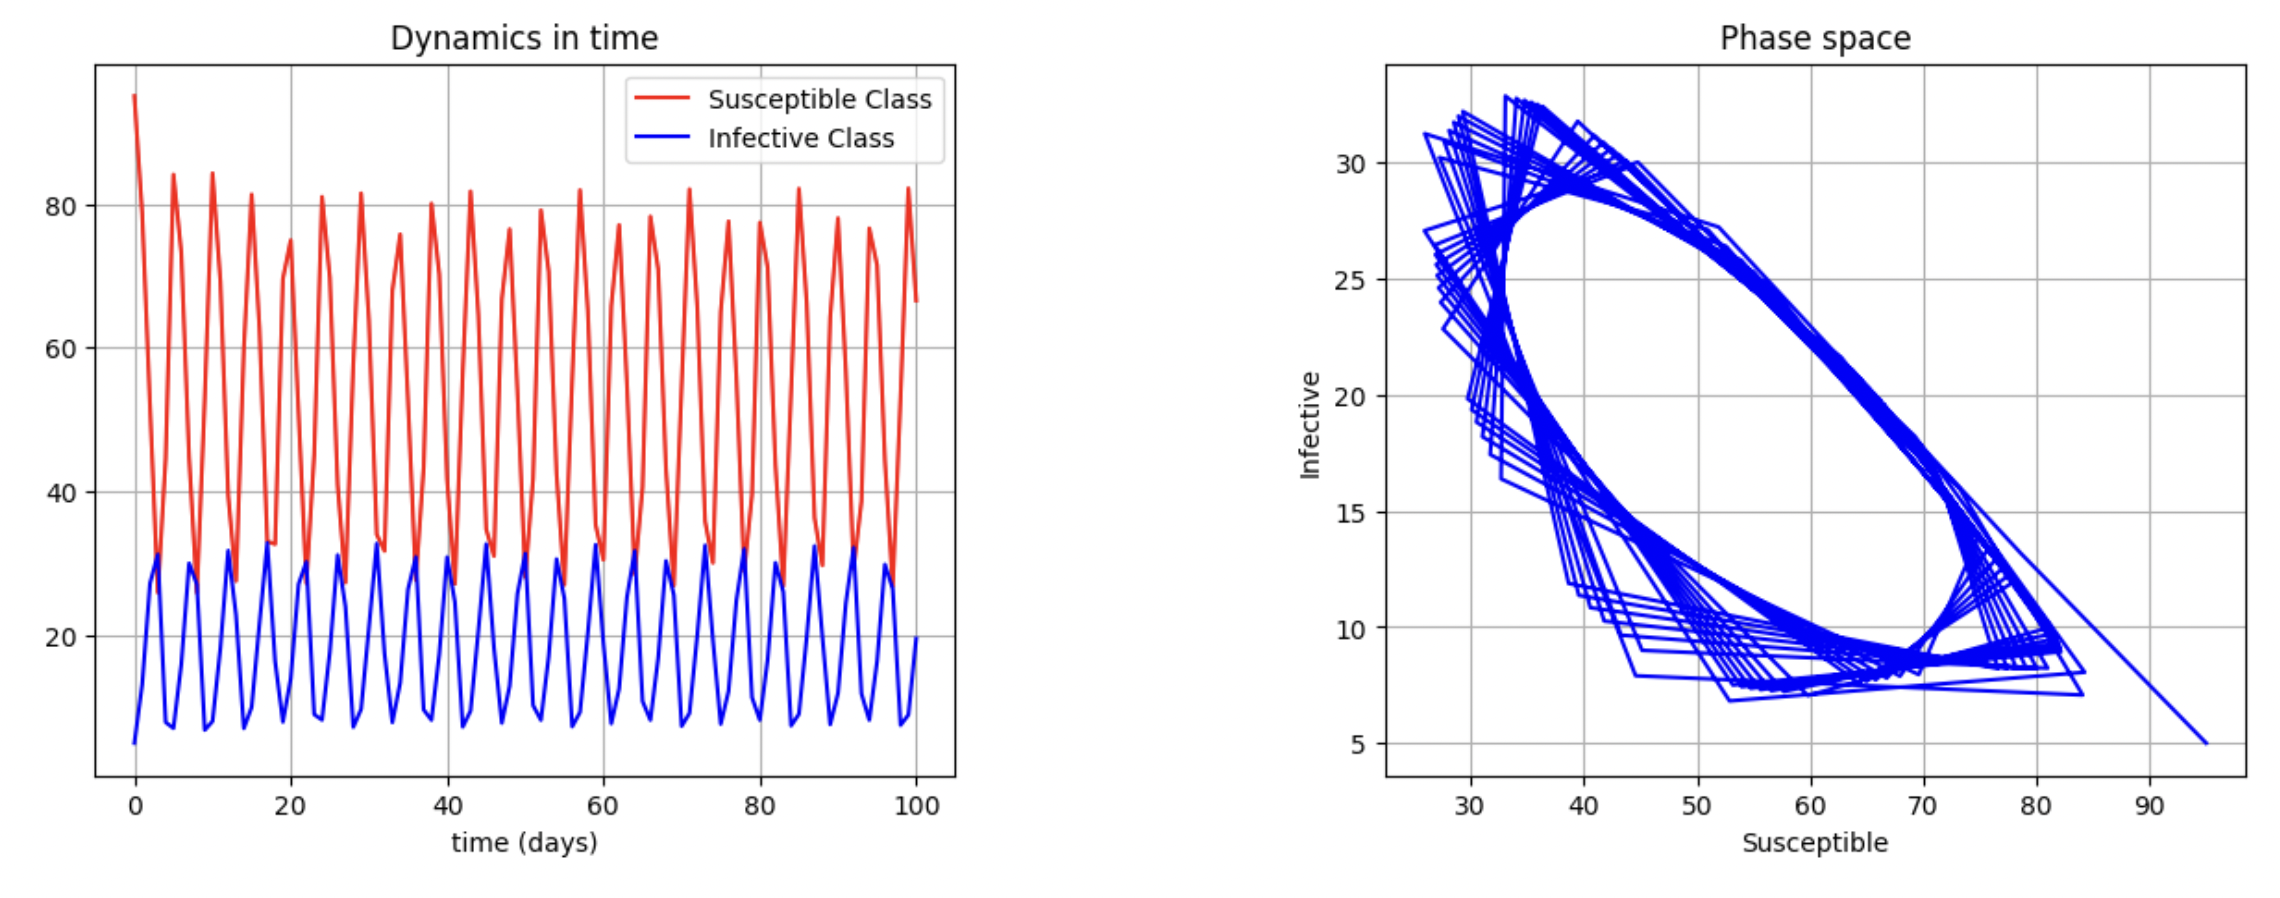
\includegraphics[width=80mm,scale=0.5]{n=100,a=.84,b=.4,d=4.5.png}
\end{figure}

Modelling subset $(N=100)$ data using $\delta = 2$, our endemic equilibrium point is $(S_e, I_e)= (47.6,20.9)$, and our following Jacobian Matrix is: 

\begin{equation}
J(S_e,I_e) = \begin{bmatrix} 
9.92 & -2.99 \\
0.79 & 1 \end{bmatrix}
\end{equation} \\

Here $T=10.9$, $D=12.3$, and $T^2-4D=70$ thus follows case 2 and our previous model, where $\lambda_1_,_2$ are real with the same sign. This model results in an unstable node. \\


\section{\label{sec:level1}Conclusions\protect\\}

Based on Covid-19 studies, people infected and recovering from Covid-19 produce an antibody response to the virus, but these antibodies decrease in a short amount of time. As the immune system relies heavily on antibodies in the defense against Covid-19, it is possible that with a decrease in antibodies, recovered patients can become reinfected in seasonal waves. Especially with varying vaccine efficacy for new Covid strains, it is important to consider immunity loss when modeling Covid disease spread. In the future, this model should also consider exposure latency time as well as birth and death rates. By creating an ODE to describe disease spread behavior, we can visualize directional changes in the system to help discover trends in the future. 


% The \nocite command causes all entries in a bibliography to be printed out
% whether or not they are actually referenced in the text. This is appropriate
% for the sample file to show the different styles of references, but authors
% most likely will not want to use it.
\nocite{*}

\bibliography{apssamp}% Produces the bibliography via BibTeX.

\end{document}
%
% ****** End of file Paper.tex ******
